\chapter{Phương pháp đề xuất}
\ifpdf
    \graphicspath{{Chapter4/Chapter4Figs/PNG/}{Chapter4/Chapter4Figs/PDF/}{Chapter4/Chapter4Figs/}}
\else
    \graphicspath{{Chapter4/Chapter4Figs/EPS/}{Chapter4/Chapter4Figs/}}
\fi

Như đã đề cập bên trên, các phương pháp phân lớp vật liệu dựa trên ảnh RGB thường dựa trên việc phân lớp đối tượng để phân loại vật liệu của chúng, điều này khiến những hệ thống này dễ phân loại sai khi những đối tượng có hình dạng hoặc texture tương tự nhau (Hình \ref{fig:shape} và \ref{fig:texture}). Nhóm đề xuất phương pháp kết hợp deep feature rút trích từ một CNN được huấn luyện sẵn (transfer learning) với các handcrafted features thích hợp trên những tập dữ liệu khác nhau (thể hiện thông tin về hình dạng và texture) để giải quyết sự nhầm lần nãy và cải thiện kết quả phân lớp (Hình \ref{fig:main_idea}). 

\begin{figure}[h!]
	\centering
	\captionsetup{width=0.75\textwidth}
	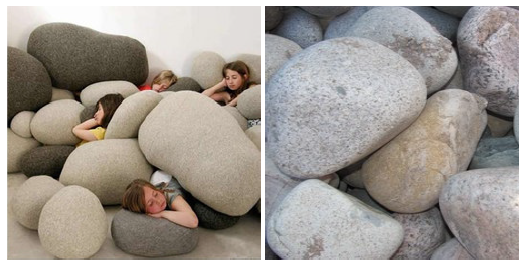
\includegraphics[width=0.8\textwidth]{shape.png}
	\caption{Các đối tượng chính của hai ảnh đều có hình dạng giống nhau và có thể bị nhầm lần cả hai đều là đá}
    \label{fig:shape}
\end{figure}

\begin{figure}[h!]
	\centering
	\captionsetup{width=0.75\textwidth}
	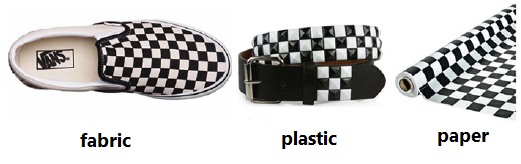
\includegraphics[width=0.8\textwidth]{texture.png}
	\caption{Các đối tượng có hình dạng khác nhau được làm từ vật liệu khác nhau nhưng lại giống nhau về texture (đều là sọc caro)}
    \label{fig:texture}
\end{figure}

\begin{figure}[h!]
	\centering
	\captionsetup{width=0.7\textwidth}
	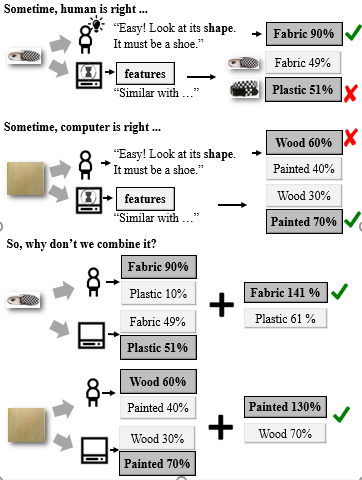
\includegraphics[width=1.0\textwidth]{main_idea.PNG}
	\caption{Deep features rút trích từ một mạng CNN đã được huấn luyện sẵn thê hiện cho cách con người học, kết hợp chúng với các handcrafted features thích hợp có thể giúp cải thiện kết quả phân lớp}
    \label{fig:main_idea}
\end{figure}

\section{Mô hình 1: kết hợp probability predictions (posfusion)}
Cấu trúc của mô hình này gồm 3 nhánh song song nhau. Nhánh thứ nhất nhận ảnh đầu vào sau đó dùng một mạng CNN được huấn luyện sẵn để rút deep feature và huấn luyện bộ phân lớp thứ 1. Nhánh thứ 2 và thứ 3 lần lượt nhận cùng ảnh đầu vào đó và dùng cái bộ lọc tương ứng để rút các thông tin về hình dạng và texture trong ảnh (handcrafted features) sau đó được dùng để huấn luyện bộ phân lớp thứ 2 và 3. 

Sau khi 3 bộ phân lớp này đã được huấn luyện, chúng được dùng để phân lớp các ảnh trong tập test và cho ra 3 kết quả khác nhau (3 vector of scores), 3 kết quả này sau đó được kết hợp với nhau để cho ra kết quả cuối cùng (Hình \ref{fig:method_1}).

\begin{figure}[h!]
	\centering
	\captionsetup{width=0.7\textwidth}
	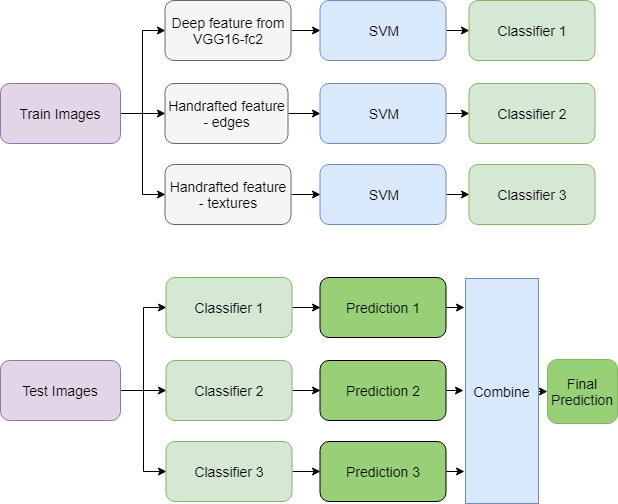
\includegraphics[width=1.0\textwidth]{method_1.png}
	\caption{Mô hình 1: kết hợp probability predictions}
    \label{fig:method_1}
\end{figure}

\section{Mô hình 2: kết hợp features (pre-fusion)}
Với mô hình này, đầu vào cũng có ba nhánh tương tự mô hình thứ nhất, tuy nhiến chúng sẽ không đi song song, thay vào đó các feature rút trích từ ba nhánh sẽ được kết hợp thành một và chỉ huấn luyện một bộ phân lớp duy nhất trên feature đã được kết hợp này.

Trong quá trình test, các feature từ 3 nhánh cũng được kết hợp tương tự và sau đó đi qua bộ phân lớp đã huấn luyện để có kết quả cuối cùng (Hình \ref{fig:method_2}).

\begin{figure}[h!]
	\centering
	\captionsetup{width=0.7\textwidth}
	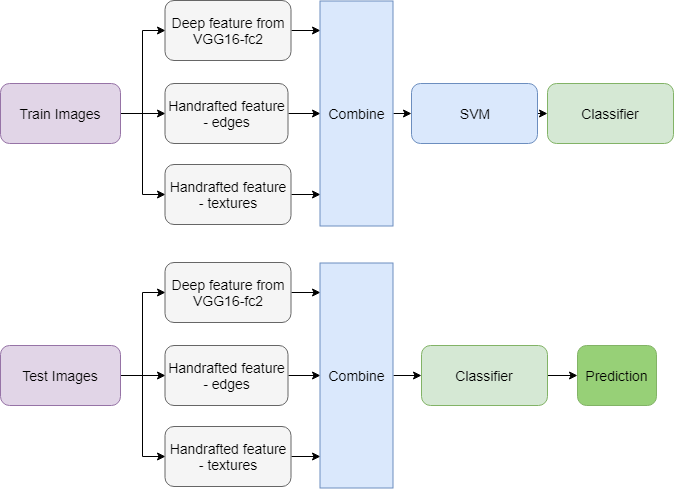
\includegraphics[width=1.0\textwidth]{method_2.png}
	\caption{Mô hình 2: kết hợp features (pre-fusion)}
    \label{fig:method_2}
\end{figure}

\section{Mô hình 3: kết hợp mô hình 1 và 2}
Mô hình này là sự kết hợp của pre-fusion và post fusion bên trên để có thể cho kết quả tốt nhất. Đầu tiên, ảnh huấn luyện sẽ được rút deep feature và các handcrafted features tương tự như trên, sau đó deep feature sẽ dùng để huấn luyện một bộ phân lớp riêng, cùng với đó, deep feature cũng sẽ được kết hợp với các handcrafted features còn lại để huấn luyện một bộ phân lớp riêng (Hình \ref{fig:method_3}).

Với mô hình này, nhánh trên (chỉ dùng deep feature) có thể coi là transfer learning từ một mạng CNN đã được huấn luyện sẵn trên ImageNet và tương ứng với cách dùng bài toán phân lớp đối tượng để giải bài toán phân lớp vật liệu, cùng với đó nhánh 2 kết hợp với các handcrafted features thích hợp sẽ giải quyết được các trường hợp nhập nhằng khi hai đối tượng có cùng hình dạng hay texture (Hình \ref{fig:shape}, \ref{fig:texture}), chính vì thế kết quả phân lớp sẽ tốt hơn.

\begin{figure}[h!]
	\centering
	\captionsetup{width=0.7\textwidth}
	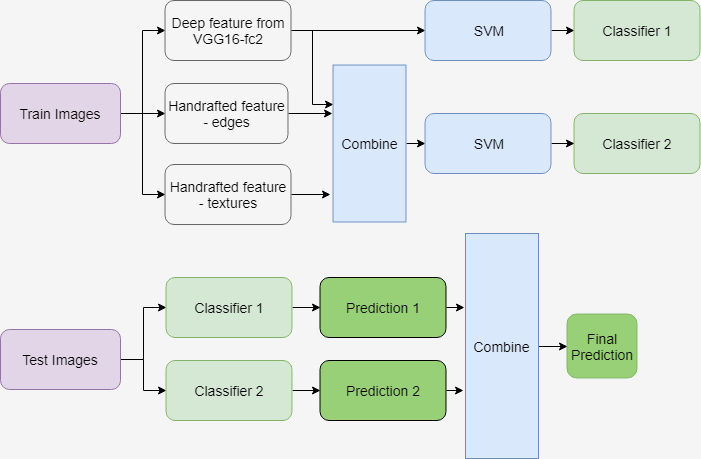
\includegraphics[width=1.0\textwidth]{method_3.png}
	\caption{Mô hình 3: kết hợp mô hình 1 và 2 (full-fusion)}
    \label{fig:method_3}
\end{figure}

\section{Thiết kế một mạng CNN duy nhất tích hợp các mô hình trên vào một}
Cách rút trích features và huấn luyện bằng SVMs như các mô hình trên 
cần lưu trữ một lượng lớn dữ liệu (các feature đã được rút trích). Bên cạnh đó quá trình huấn luyện (bằng SVMs) mất rất nhiều thời gian, tuy nhiên để có một kết quả tốt nhóm cần phải thử nghiệm với rất nhiều bộ tham số khác nhau (của SVMs) nên thời gian và khối lượng tính toán không hề nhỏ, thêm vào đó các bộ phân lớp sau khi đã huấn luyện không thể dùng lại trong lần huấn luyện sau. Thế nên, nhóm đã đề xuất phương pháp kết hợp các mô hình trên vào một mạng CNN duy nhất. Mục tiêu được đề ra là với mạng CNN nhóm sẽ có thể:
\begin{enumerate}
	\item Gộp cả 3 quá trình rút trích feature, huấn luyện và test vào một quá trình duy nhất là huấn luyện mạng CNN này.
	\item Giảm chi phí (không gian lưu trữ, khối lượng và thời gian tính toán)
	\item Khả năng mở rộng và sử dụng lại: mạng CNN có khả năng tự thay đổi tham số để thích ứng tốt hơn với dữ liệu mới (các bộ phân lớp của SVMs thì không thể).
    
Ý tưởng chung của mạng được trình bày trong Hình \ref{}
\end{enumerate}